\documentclass[a4paper,11pt]{article}

% Kodovani (cestiny) v dokumentu: utf-8
%\usepackage[cp1250]{inputenc}	% Omezena stredoevropska kodova stranka, pouze MSW.
\usepackage[utf8]{inputenc}	% Doporucujeme pouzivat UTF-8 (unicode).

\usepackage[margin=2cm]{geometry}
\newtoks\jmenopraktika \newtoks\jmeno \newtoks\datum
\newtoks\obor \newtoks\skupina \newtoks\rocnik \newtoks\semestr
\newtoks\cisloulohy \newtoks\jmenoulohy
\newtoks\tlak \newtoks\teplota \newtoks\vlhkost

\jmenopraktika={Fyzikální praktikum 1}
\jmeno={Lukáš Lejdar}
\datum={16. dubna 2024}
\obor={F}
\skupina={Út 16:00}

\cisloulohy={3}
\jmenoulohy={Měření viskozity, hustoty a povrchového napětí kapalin}
\tlak={101{,}35}
\teplota={22,4}
\vlhkost={47,7}

%%%%%%%%%%% Uzitecne balicky:
\usepackage[czech]{babel}

\usepackage{graphicx}
\usepackage{amsmath}
\usepackage{xspace}
\usepackage{url}
\usepackage{indentfirst}
\usepackage{wrapfig}
\usepackage{subcaption}
\usepackage{xcolor}

%%%%%% Zamezeni parchantu:
\widowpenalty 10000 \clubpenalty 10000 \displaywidowpenalty 10000
%%%%%% Parametry pro moznost vsazeni vetsiho poctu obrazku na stranku
\setcounter{topnumber}{3}	  % max. pocet floatu nahore (specifikace t)
\setcounter{bottomnumber}{3}	  % max. pocet floatu dole (specifikace b)
\setcounter{totalnumber}{6}	  % max. pocet floatu na strance celkem
\renewcommand\topfraction{0.9}	  % max podil stranky pro floaty nahore
\renewcommand\bottomfraction{0.9} % max podil stranky pro floaty dole
\renewcommand\textfraction{0.1}	  % min podil stranky, ktery musi obsahovat text
\intextsep=8mm \textfloatsep=8mm  %\intextsep pro ulozeni [h] floatu a \textfloatsep pro [b] or [t]

% Tecky za cisly sekci:
\renewcommand{\thesection}{\arabic{section}.}
\renewcommand{\thesubsection}{\thesection\arabic{subsection}.}
% Jednopismenna mezera mezi cislem a nazvem kapitoly:
\makeatletter \def\@seccntformat#1{\csname the#1\endcsname\hspace{1ex}} \makeatother
%
\newcommand{\vsn}[4]{\ensuremath{#1 =} #2(#3)\,#4}
\newcommand{\vrn}[6]{\ensuremath{#1 =} (#2 $\pm$ #3)\,#4 ($p=$ #5\,\%, $\nu=$ #6)}


%%%%%%%%%%%%%%%%%%%%%%%%%%%%%%%%%%%%%%%%%%%%%%%%%%%%%%%%%%%%%%%%%%%%%%%%%%%%%%%
% Zacatek dokumentu
%%%%%%%%%%%%%%%%%%%%%%%%%%%%%%%%%%%%%%%%%%%%%%%%%%%%%%%%%%%%%%%%%%%%%%%%%%%%%%%

\begin{document}

\thispagestyle{empty}

{
\begin{center}
\sf 
{\Large Ústav fyziky a technologií plazmatu Přírodovědecké fakulty Masarykovy univerzity} \\
\bigskip
{\huge \bfseries FYZIKÁLNÍ PRAKTIKUM} \\
\bigskip
{\Large \the\jmenopraktika}
\end{center}

\bigskip

\sf
\noindent
\setlength{\arrayrulewidth}{1pt}
\begin{tabular*}{\textwidth}{@{\extracolsep{\fill}} l l}
\large {\bfseries Zpracoval:}  \the\jmeno & \large  {\bfseries Naměřeno:} \the\datum\\[2mm]
\large  {\bfseries Obor:} \the\obor  \hspace{40mm}  {\bfseries Skupina:} \the\skupina %
&\large {\bfseries Testováno:}\\
\\
\hline
\end{tabular*}
}

\bigskip

{
\sf
\noindent \begin{tabular}{p{4cm} p{0.6\textwidth}}
\Large  Úloha č. {\bfseries \the\cisloulohy:} \par
\smallskip
$T=\the\teplota$~$^\circ$C \par
$p=\the\tlak$~kPa \par
$\varphi=\the\vlhkost$~\%
&\Large \bfseries \the\jmenoulohy  \\[2mm]
\end{tabular}
}

\vskip1cm

\section{Úvod}

Úloha je zaměřená na základní mechanické vlastnosti kapalin a metody jejich měření. Pokusím~se~ty nejdůležitější veličiny nejdřív krátce shrnout. \\

I v kapalině probíhá efekt podobný tření. Molekuly proudící blízko sebe spolu různě interagují a mají tendenci svoji rychlost srovnávat. Tento efekt popisuje Newtonův zákon pro laminárně proudící kapaliny zavedením \textbf{dynamické viskozity} $\eta$, jako konstantu přímé úměry

\begin{equation}
  \tau = \eta \frac{dv_x}{dy},
\end{equation}

kde $\tau$ je smykové napětí mezi vrstvami kapaliny a  $\frac{dv_x}{dy}$ je derivace rychlosti proudění kapaliny ve
směru normály k rovině smykového napětí $\tau$. S dynamickou viskozitou se často setkáme v podílu s hustotou kapaliny. Konvenčně tuto veličinu definujeme jako \textbf{Kinematickou viskozitu} $\nu$

\begin{equation}
\nu = \frac{\eta}{\rho}
\end{equation}

Další důležitou vlastností kapalin je tzv. \textbf{povrchové napětí} $\sigma$. Definujeme ho jako sílu působící v rovině povrchu kapaliny, kolmo na libovolnou délkovou jednotku v povrchu kapaliny, vztaženou na tuto délku.

\begin{equation}
  \sigma = \frac{F}{L}
\end{equation}

Podle Fowkese a van Osse et al. působí v povrchové vrstvě různé mezimolekulární síly, které aditivně přispívají k celkovému povrchovému napětí. Většinu z nich lze zahrnout do dvou větších kategorií acidobazických interakcí a Van der Walsových sil.

\begin{equation}
  \sigma = \sigma^{\text{lw}} + \sigma^{\text{ab}}
\end{equation}

\newpage

\section{Teorie}

\subsection{Absolutní měření viskozity kapalin}

Pokud kapalina proudí v kapiláře laminárně, platí zjednodušený tvar Hagenovy – Poiseuillovy rovnice

\begin{equation}
\frac{dV}{dt} =  \bar{v} \pi R^2 = \frac{\pi R^4 \Delta p }{8 \eta L} 
\end{equation}

\noindent
kde $\Delta$p je tlakový spád mezi konci trubice, L délka trubice, R poloměr trubice a $\frac{dV}{dt}$ okamžitý průtokový objem. Mariottova láhev z obrázku 1 dokáže zajistit stálý tlakový spád, čímž se vztah dál zjednoduší na tvar

\begin{equation}
\eta = \frac{\pi R^4 \Delta p t}{8 V L}.
\end{equation}

\begin{figure}[htpb]
  \centering
  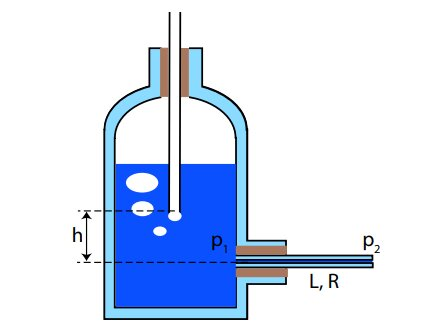
\includegraphics[width=0.4\textwidth]{mariottova_lahev.jpg}
  \caption{Mariottova láhev s kapilárou pro absolutní měření viskozity.}
\end{figure}

\subsection{Ubbelohdeho viskozimetr}

Ubbelohdeho viskozimetr na obrázku 2 je právě připravený k měření. Na kapiláře se díky trubici~A vytváří tlakový rozdíl $\Delta p$ = $h(t) \rho g + p_{Atm} - p_{Atm}$ a kapalina z trubice B tak může protékat do spodních baněk. Pokud je proudění laminární, platí opět Poiseuillův vztah (4).

\begin{figure}[htpb]
  \centering
  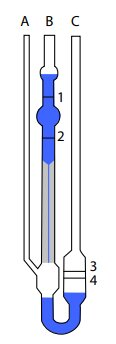
\includegraphics[width=0.13\textwidth]{ubbelhdeh.jpg}
  \caption{Ubbelohdeho kapilární viskozimetr}
\end{figure}

Uvažujme časový interval od momentu $t_1$, kdy hladina v trubici B míjí rysku 1 do chvíle $t_2$, kdy míjí rysku 2. 

\begin{align}
  \eta \frac{dV}{dt} &= \frac{\pi R^4}{8 L} \Delta p \\
  \eta A(h) dh &= \frac{\pi R^4}{8 L} h \rho g dt \\
  \frac{\eta}{\rho} \int_{h_1}^{h_2} \frac{A(h)}{h} dh &= \frac{\pi R^4}{8 L} g \int_{t_1}^{t_2} dt 
\end{align}

Všechny konstanty vystupující na pravé straně jsou nezávislé na vlastnostech měřené kapaliny, stejně jako Integrál na straně levé. Můžu psát

\begin{equation}
\nu = K(t_2-t_1),
\end{equation}

kde $\nu$ je kinematická viskozita, $t_2-t_1$ čas za který odteče kapalina od rysky 1 k rysce 2 a K časová konstanta viskozimetru. Časovou konstantu je pro měření nejdřív potřeba zkalibrovat pomocí kapaliny se známou kinematickou viskozitou.

\subsection{Měření povrchového napětí du Noüyho metodou}

Du Noüyho metoda spočívá v měření síly působící podél obvodu ponořeného objektu. Na podvěsné váhy pověsím železný kroužek, váhy vytáruji a pod kroužek položím misku s kapalinou na desku s vertikálním posuvem. Misku začnu pomalu zvedat, dokud se celý kroužek neponoří a pak ji zase pomalu vytahuji. Celý proces by měl probíhat jako na obrázku 3.

\begin{figure}[htpb]
  \centering
  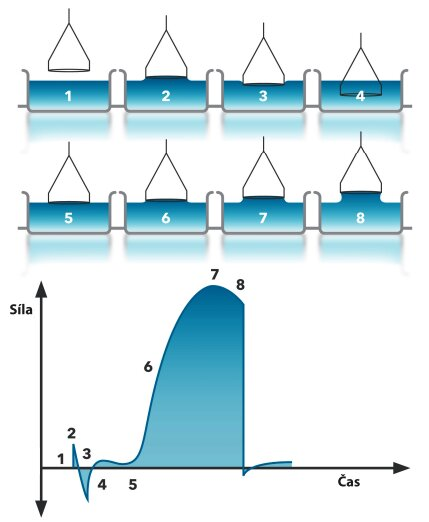
\includegraphics[width=0.4\textwidth]{nouyh.jpg}
  \caption{Závislost síly působící na kroužek při jeho ponoru a vytahování. Převzato
z http://www.attension.com}
\end{figure}

Povrchové napětí bude odpovídat největší síle kterou dokázala kapalina působit na délku kroužku

\begin{equation}
\sigma = \frac{F_{\text{max}}}{4 \pi R} \cdot f (\frac{R^3}{V}, \frac{R}{r}),
\end{equation}

\noindent
kde R je poloměr kroužku a $f (\frac{R^3}{V}, \frac{R}{r})$ HarkinsůvJordanův korekční faktor, který je tabelován pro bezrozměrné veličiny $\frac{R^3}{V}$ a $\frac{R}{r}$ ; $V=\frac{F_{\text{max}}}{(\rho - \rho_v)g}$ a r je poloměr drátku.

\subsection{Měření hustoty metodou ponorného tělíska}

Tato metoda využívá Archimedova zákona pro měření hustoty kapaliny. Změříme vztlak působící na plně ponořené těleso v kapalině o známé hustotě a v kapalině s neznámou hustotou. Výslednou hodnotu získáme ze vztahu

\begin{equation}
  \rho = \frac{m}{m_{\text{známé}}} \rho_{\text{známé}}
\end{equation}

\subsection{Měření hustoty pyknometrem}

Pyknometr je skleněná nádoba, kterou lze naplnit velmi přesným, ale neznámým objemem kapaliny. Zvlášť zvážím hmotnost m prázdného pyknometru, hmotnost $m_1$ pyknometru naplněného kapalinou o neznámé hustotě $\rho_1$ a hmotnost $m_2$ pyknometru naplněného kapalinou o známé hustotě $\rho_2$.

\begin{equation}
  \rho_1 = (\rho_2 - \rho_{\text{vzduchu}}) \frac{m_1 - m}{m_2 - m} + \rho_{\text{vzduchu}}
\end{equation}

\subsection{Měření složek povrchového napětí metodou kontaktního úhlu přisedlé kapky}

Povrchové napětí nejčastěji měříme na rozhraní kapalina - vzduch, jelikož vzduch nereaguje ani s kapalinou, ani sám se sebou. Nevznikne žádný příspěvek od molekul vzduchu a nic neoponuje přitažlivým silám mezi molekulami kapaliny, které se tím v součtu projeví všechny. Dupreho rovnice (14) naopak popisuje případ, kdy obě látky na rozhraní mají vlastní povrchové napětí $\sigma_s$,  $\sigma_l$ a zároveň spolu interagují.

\begin{equation}
  \sigma_{\text{sl}} =
  \sigma_{\text{s}} + \sigma_{\text{l}} - 2 \sqrt{\sigma_{\text{s}}^{\text{lw}}\sigma_{\text{l}}^{\text{lw}}} - 2\sqrt{\sigma_{\text{s}}^{\text{ab}}\sigma_{\text{l}}^{\text{ab}}} \\
\end{equation}

Cílem měření je zjistit, jak se známá hodnota povrchového napětí $\sigma_{\text{l}}$ rozkládá do složek $\sigma_{\text{l}}^{\text{lw}}$, $\sigma_{\text{l}}^{\text{ab}}$ ze vztahu (4) a jak bude podle vztahu (14) reagovat s jinými materiály.  Kapka nanesená na vhodný povrch jako na obrázku~4, je právě co hledáme. Pro úhel $\theta$, který svírá tečna k profilu kapky v místě styku všech tří fází platí Youngova rovnice \\

\begin{equation}
\sigma_{\text{s}} = \sigma_{\text{sl}} + \sigma_{\text{l}}\cos(\theta),
\end{equation}

\noindent
kde $\sigma_{\text{l}}$ a $\sigma_{\text{s}}$ jsou povrchové mezifázové energie kapaliny a pevné látky vůči páře kapaliny a $\sigma_{\text{sl}}$ mezifázová povrchové energie rozhraní kapalina – pevná látka.

\begin{figure}[htpb]
  \centering
  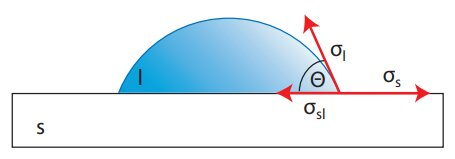
\includegraphics[width=0.5\textwidth]{young.jpg}
  \caption{Youngova rovnováha na rozhraní tří fází u přisedlé kapky}
\end{figure}

Kombinací Youngovy a Dupreho rovnice dostaneme rovnici Youngovu-Dupreho:

\begin{equation}
  (1 + \cos(\theta))\sigma_{\text{l}} =  2 \sqrt{\sigma_{\text{s}}^{\text{lw}}\sigma_{\text{l}}^{\text{lw}}} + 2\sqrt{\sigma_{\text{s}}^{\text{ab}}\sigma_{\text{l}}^{\text{ab}}}
\end{equation}

Abychom změřili jen jednu složku povrchového napětí, musíme ji nějak izolovat od té druhé. Teflon má například povrchovou energii pouze disperzního charakteru, tj. $\sigma_{\text{s}} = \sigma_{\text{s}}^{\text{lw}}$ a na pravé straně rovnice zbude jediná odmocnina. Dál můžeme jako kalibrační kapalinu použít metylenjodid (CH$_{2}$I$_{2}$), který má povrchovou energii rovněž čistě disperzního charakteru.

\begin{align}
  (1 + \cos\theta_{\text{H}_2\text{O}}) \sigma_{\text{H}_2\text{O}} &= 2 \sqrt{\sigma_{\text{s}}^{\text{lw}} \sigma_{\text{H}_2\text{O}}^{\text{lw}}} \\
  (1 + \cos\theta_{\text{kal}}) \sigma_{\text{kal}} &= 2 \sqrt{\sigma_{\text{s}}^{\text{lw}} \sigma_{\text{kal}}}
\end{align}

Po vydělení obou rovnic dostávám pro disperzní složku povrchové energie vody

\begin{equation}
\sigma^{lw}_{\text{H}_2\text{O}} =
\frac{ (\sigma_{\text{H}_2\text{O}})^2 }{ \sigma_{\text{kal}} }
\left( \frac{1 + \cos \theta_{\text{H}_2\text{O}}}{ 1 + \cos \theta_{\text{kal}} } \right)^2
\end{equation}

\section{Výsledky měření}

\subsection{Absolutní měření viskozity Mariottovou lahví}

Za dobu t = 128 s vytekl kapilárou objem V = $38.2 \pm 3$ cm$^{3}$ destilované vody. Uvádím taky parametry použité Mariottovy láhve pro výpočet dynamické viskozity ze vztahu (6).
\begin{flalign*}
  & \text{poloměr kapiláry} & R &= 0.570 \pm 0.001 \text{ mm} &  \\
  & \text{délka kapiláry} & L &= 165.0 \pm 0.5 \text{ mm} & \\
  & \text{tlakový spád} & \rho &= 1110 \pm 40 \text{ Pa} &
\end{flalign*}

\begin{equation*}
  \eta = 1.03 \pm 0.01 \cdot 10^{-3} \text{ mPas}
\end{equation*}

\subsection{Měření Ubbelohdeho viskozimetrem}

Laboratorní viskozimetr už je zkalibrovaný pro hodnotu K

\begin{equation*}
K = 1.063 \pm 0.0069 \cdot 10^{-9} \text{ m}^{2}\text{s}^{-2}.
\end{equation*}

Provedl jsem 3 měření kinematické viskozity vody. Jedno při laboratorní teplotě a dvě po ponoření celého viskozimetru v ohřáté vodě. Naměřené hodnoty jsou uvedené v tabulce 1 a kinematickou viskozitu jsem spočítal ze vztahu  (6). \\

\begin{table}[h]
    \centering
    \begin{tabular}{ | c | c | c | c |}
    \hline
    $T$ (°C) & $t$ (m:s) & $\nu_{\text{H}_2\text{O}}$ (mm$^{2}$s$^{-1}$) & tabulkové $\nu_{\text{H}_2\text{O}}$ (mm$^{2}$s$^{-1}$) \\\hline
    25 & 14:22 & 0.916 $\pm$ 0.006 & 0.8926 \\
    30 & 12:25 & 0.792 $\pm$ 0.005  & 0.8007 \\
    35 & 11:23 & 0.726 $\pm$ 0.005 & 0.7234 \\\hline
    \end{tabular}
    \caption{Změřené hodnoty kinematické viskozity pro různé teploty}
\end{table}

\subsection{Měření hustoty metodou ponorného tělíska}

Na závěsných vahách jsem změřil vztlak ponořeného tělíska v destilované vodě a v lihu. Hustotu dopočítám ze vztahu (12).
\begin{flalign*}
  & \text{tíha tělíska ponořeného v lihu} & m_{\text{l}} &= 36.37 \pm 0.03 \text{ mN} \\
  & \text{tíha tělíska ponořeného ve vodě} & m_{\text{v}} &= 41.08 \pm 0.03 \text{ mN} & \\
  & \text{hustota destilované vody} & \rho_{\text{v}} &= 997 \text{ kgm}^{-3} &
\end{flalign*}
\begin{equation*}
  \rho_{\text{l}} = 804.4 \pm 0.9 \text{ kgm}^{-3}
\end{equation*}
\subsection{Měření hustoty pyknometrem}

Ze vztahu (13) dopočítám hustotu lihu $\rho_{\text{l}}$, pomocí známé hustoty destilované vody $\rho_{\text{v}} = 997$ kgm$^{-3}$.
\begin{flalign*}
  & \text{hmotnost prázdného pyknometru} & m &= 17.728 \pm 0.003\ g & \\
  & \text{hmotnost pyknometru s lihem} & m_\text{l} &= 38.580 \pm 0.003\ g & \\
  & \text{hmotnost pyknometru s destilovanou vodou} & m_{\text{v}} &=  43.740 \pm 0.003\ g & \\
  & \text{hustota vzduchu v laboratoři} & \rho_{\text{vz}} &= 1.204 \text{ kgm}^{-3}
\end{flalign*}
\begin{equation*}
\rho_{\text{l}} = 799.5 \pm 0.2 \text{ kgm}^{-3}
\end{equation*}

\subsection{Měření povrchového napětí du Noüyho metodou}

Celkem jsem pro každou kapalinu udělal 10 měření a výsledky i s nejistotou uvedl v tabulce 2. Poloměr kroužku byl R$= 29.0 \pm 0.05$ mm a Harkinsův-Jordanův korekční faktor f = 0.77.


\begin{table}[htpb]
  \centering
  \begin{tabular}{| c | c | c |}
    \hline
    kapalina & $F_{max}$ (mN) & $\sigma$ (mNm$^{-1}$) \\\hline
    líh & 12.01 $\pm$ 0.2 & 25.4 $\pm$ 0.5 \\
    destilovaná voda & 34.42 $\pm$ 0.2 & 72.7 $\pm$ 0.5 \\ \hline
  \end{tabular}
  \caption{Povrchové napětí destilované vody a lihu}
\end{table}

\vspace{-10pt}

\subsection{Měření složek povrchového napětí metodou kontaktního úhlu přisedlé kapky}

\begin{figure}[htpb]
  \centering
  \begin{subfigure}[b]{0.45\textwidth}
    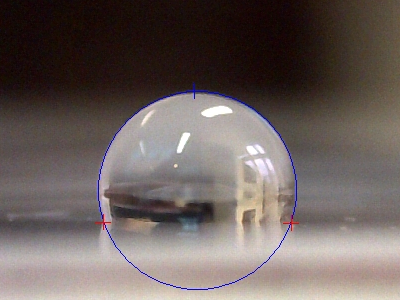
\includegraphics[width=\textwidth]{kapky/voda_001p_crop.jpg}
    \caption{Destilovaná voda}
  \end{subfigure}
  \hfill
  \begin{subfigure}[b]{0.45\textwidth}
    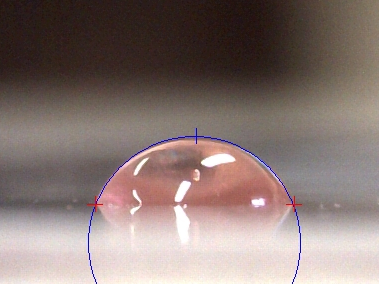
\includegraphics[width=\textwidth]{kapky/voda_002p_crop.jpg}
    \caption{metylenjodid}
  \end{subfigure}
  \caption{Kapky přisedlé na teflonové podložce}
\end{figure}

Disperzní složku povrchového napětí vody dopočítám ze vztahu (19).

\begin{flalign*}
  & \text{povrchové napětí metylenjodidu} & \sigma_{\text{kal}} &= 50.8 \text{ Nm}^{-1} & \\
  & \text{povrchové napětí destilované vody} & \sigma_{\text{v}} &= 72.8 \text{ Nm}^{-1} & \\
  & \text{změřený úhel přisedlé kapky metylenjodidu} & \theta_{\text{v}} &= 68.7 ^{\circ} & \\
  & \text{změřený úhel přisedlé kapky vody} & \theta_{\text{v}} &= 109.5 ^{\circ} &
\end{flalign*}

\begin{align*}
  \sigma^{lw}_{\text{H}_2\text{O}} &= 24.9 \text{ Nm}^{-1} & \sigma^{ab}_{\text{H}_2\text{O}} = \sigma_{\text{H}_2\text{O}} - \sigma^{lw}_{\text{H}_2\text{O}} &= 47.9 \text{ Nm}^{-1} \\
\end{align*}

\section{Závěr}

Pomocí Mariottovy lahve jsem změřil jsem dynamickou viskozitu destilované vody o teplotě 22~$^{\circ}$C $\eta = (1.03 \pm 0.01) \text{ mPas}$. Tabulky udávají pro tuto teplotu hodnotu 0.9544 mPas. Chybu mohlo způsobit nepřesné měření času, nebo objemu vody, který vytekl kapilárou. \\

Ubbelohdeho viskozimetrem jsem změřil kinematickou viskozitu vody o teplotě 25 $^{\circ}$C, 30 $^{\circ}$ C a 35~$^{\circ}$C. Výsledky jsou uvedené v tabulce 1 a dobře odpovídají tabulkovým hodnotám z odkazu 1. \\

Určil jsem hustotu lihu zvlášť metodou ponorného tělíska $\rho = 804.4 \pm 0.9 \text{ kgm}^{-3}$ a pyknometrem $\rho = 799.5 \pm 0.2 \text{ kgm}^{-3}$, oproti tabulkové hodnotě 789 kgm $^{-3}$. Pyknometr jsem trochu přelil a zůstala na něm nějaké kapaky, které mohli způsobit chybu měření. V případě ponorného tělíska je možné, že jsem ho při ponoru do kalibrační kapaliny neponořil stejně jako do lihu, což by mohlo způsobit rozdíl hodnot.\\

Du Noüyho metodou jsem změřil povrchové napětí lihu $\sigma = 25.4 \pm 0.5$ mNm$^{-1}$ a destilované vody $\sigma = 72.7 \pm 0.5$~mNm$^{-1}$. Nejistotu obou hodnot tvoří převážně nejistota velikosti poloměru kroužku a korekčního faktoru. Mám ale pořád velmi dobrou shodu s tabulkovými hodnotami 22.4 a 72.8 mNm$^{-1}$. Malou chybu povrchového napětí lihu pravděpodobně způsobily nečistoty v nádobě. \\

Měřením kontaktního úhlu kapky destilované vody přisedlé na podložce z teflonu jsem určil složky povrchového napětí $\sigma^{lw} = 24.9 \text{ mNm}^{-1}$ a $\sigma^{ab} = 47.9 \text{ mNm}^{-1}$. Tabulkové hodnoty jsou 21.8 a 51.0~mNm$^{-1}$. I tady výsledek mohly ovlivnit malé nečistoty na podložce.


\begin{thebibliography}{0}
\bibitem{tabulky} Kinematická a dynamická viskozita vody ~\url{https://wiki.anton-paar.com/en/water/}.   
\end{thebibliography}

\end{document}
